\documentclass[prd,preprintnumbers,onecolumn,eqsecnum,floatfix,letter]{revtex4}
\usepackage{color}
\usepackage{calc}
\usepackage{amsmath,amssymb,graphicx}
\usepackage{amssymb,amsmath}
\usepackage{tensor}
\usepackage{bm}
\usepackage{times}
\usepackage[varg]{txfonts}
\usepackage{mathrsfs,amsmath}  
\usepackage{empheq}
\usepackage[colorlinks, pdfborder={0 0 0}]{hyperref}
\definecolor{LinkColor}{rgb}{0.75, 0, 0}
\definecolor{CiteColor}{rgb}{0, 0.5, 0.5}
\definecolor{UrlColor}{rgb}{0, 0, 0.75}
\hypersetup{linkcolor=LinkColor}
\hypersetup{citecolor=CiteColor}
\hypersetup{urlcolor=UrlColor}
\maxdeadcycles=1000
\allowdisplaybreaks
\textwidth 7.5 in 
\hoffset -1 cm 
\newcommand{\boxedeq}[2]{\begin{empheq}[box={\fboxsep=6pt\fbox}]{align}\label{#1}#2\end{empheq}}
\newcommand{\comment}[1]{\textcolor{blue}{\textit{#1}}}
\newcommand{\Sean}[1]{\textcolor{red}{\textit{Sean:#1}}}
\newcommand{\ashok}[1]{\textcolor{cyan}{\textit{Ashok:#1}}}


\begin{document}

\newcommand{\be}{\begin{equation}}
\newcommand{\ee}{\end{equation}}
\newcommand{\ber}{\begin{eqnarray}}
\newcommand{\eer}{\end{eqnarray}}
\def\bea{\begin{eqnarray}}
\def\eea{\end{eqnarray}}
\newcommand{\etal}{\emph{et al.}}


\title{Notes on applying super momentum balance law to constraint GW waveform }
\author{Ashok Choudhary}\email{aschoudhary@mix.wvu.edu}
\author{Sean T. McWilliams}\email{sean.mcwilliams@mail.wvu.edu}
\affiliation{Department of Physics and Astronomy, West Virginia University, Morgantown, WV 26506, USA}

\begin{abstract}
\end{abstract}

\maketitle

\section{Local super momentum balance law}


\begin{equation}
\mathcal{F}(\theta,\phi) \Big|^{u_{2}}_{u_{1}}  := -\int_{u_{1}}^{u_{2}} du \left[|\dot{\sigma^{o}}|^{2} - \Re\left(\eth^{2}\dot{\bar{\sigma}}^{o} \right) \right](u, \theta, \phi) = \Re\left[\Psi^{o}_{2} + \bar{\sigma}^{o}\dot{\sigma^{o}}\right]\left(u_{1}, \theta, \phi\right) - \Re\left[\Psi^{o}_{2} + \bar{\sigma}^{o}\dot{\sigma^{o}}\right]\left(u_{2}, \theta, \phi\right) 
\end{equation}
where
\begin{align}
	2 \Re\, \Psi^{o}_{2}\left(u, \theta, \phi \right) & = \lim_{r \to +\infty} r^{3} \, C_{abcd}n^{a}l^{b}n^{c}l^{d}\label{psi2}\\  \Psi^{o}_{4}\left(u, \theta, \phi \right) & = \lim_{r \to +\infty} r \, C_{abcd}n^{a}\bar{m}^{b}n^{c} \bar{m}^{d} = \ddot{\bar{\sigma}}^{o} = r\left(\ddot{h}_{+} + i\, \ddot{h}_{\times}  \right)
	\label{psi4}
\end{align}
\section{ Weyl scalar $\Psi^{o}_{2}$ for BOB as perturber cross the light ring }
In Backwards One-Body (BOB)[add ref] description of black hole binary merger, the system is described as a single black hole spacetime with a inspiraling in perturber. The $\Psi^{o}_{2}$ for the unperturbed Kerr space time is given by $\Psi^{o}_{2} = M\,\rho^{3}$, where $\rho = - (r - i\,a\, \cos\theta)^{-1}$. Here we consider the modification to caused by a point particle orbiting in equatorial plain. The leading order correction (stationary and axis symmetric) to $\Psi^{o}_{2}$ for Kerr spacetime due to presence of such perturber  is done by MERLIN, ORI, BARACK, POUND, and VAN DE MEENT [add ref] in ingoing radiation gauge. Since we need the asymptotic limit \ref{psi2} in the super momentum balance law, the only use full part in our of their results in given in equation 58 in ref [add ref]    
\begin{figure}
	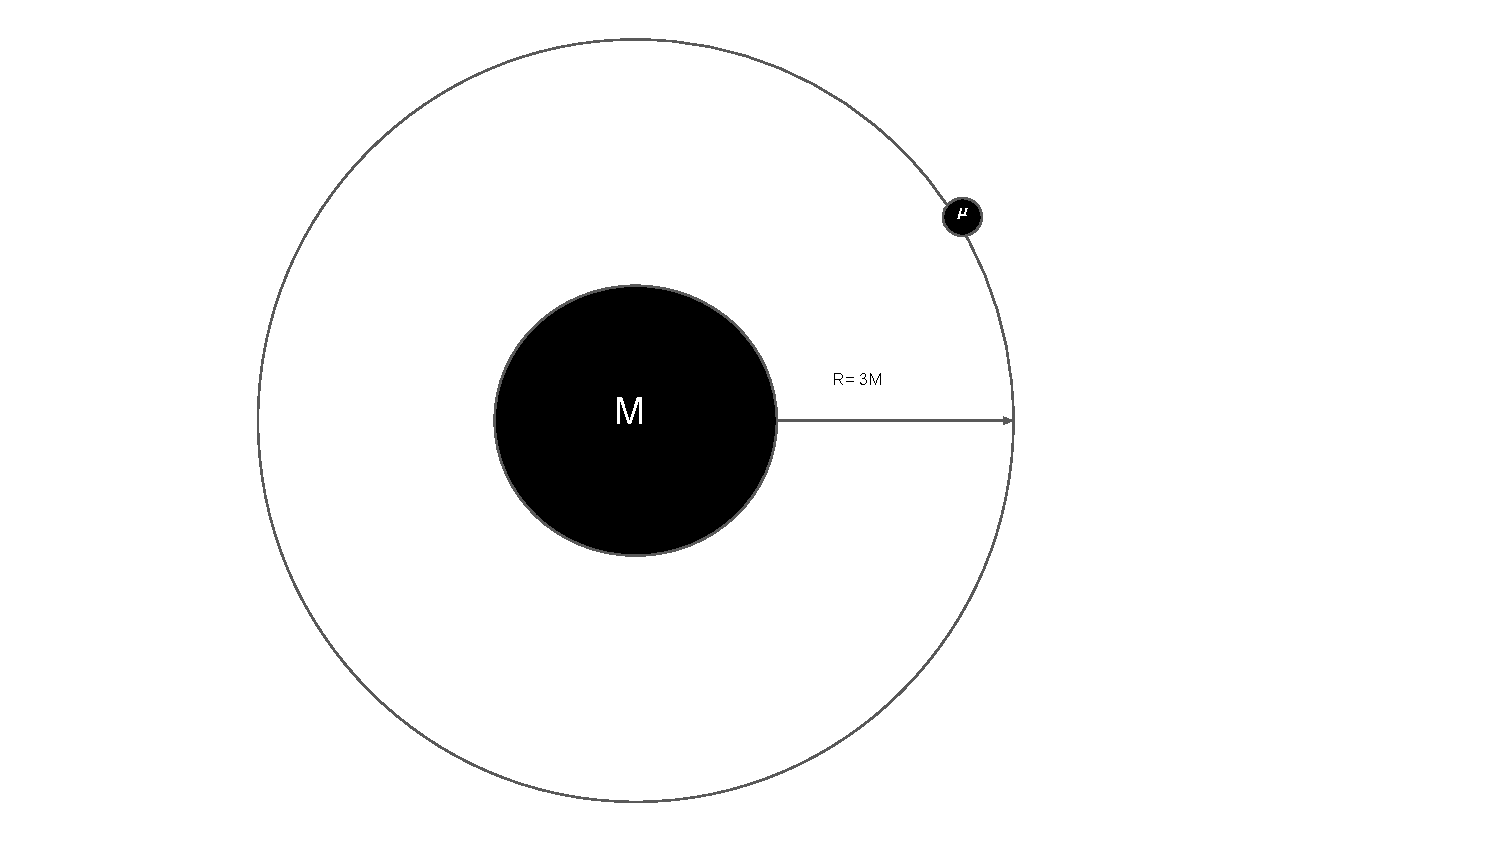
\includegraphics[width=5.5in]{../plots/BOB.pdf}
	\caption{The figure}
	\label{fig:resedualGrowthLogLog}
\end{figure} 
\subsection{Asymptotic axial and asymmetric part of $\Psi^{o}_{2}$ for perturbed black hole }
\begin{align}
	\Psi_{2}  = \Psi^{(0)}_{2} + 	\Psi^{(1)}_{2} \nonumber \\
	 \, \Psi^{(0)}_{2}  = M\,\rho^{3} \, \nonumber \\ \text{and} \, \Psi^{(1)}_{2}  = \frac{E}{r^{3}},\\ \space E := -\mu\, u_{t} = \mu\frac{(1- 2 M/r_{0})}{(1- 3M/r_{0})^{1/2}}
\end{align}
The radiation reaction has a negligible effect on dynamics of the perturber inside ISCO, so we model the rate of mass loss to the $\Psi^{o}_{2}$. First we observe  the the luminosity of gravitational wave from binary system is given by
\begin{equation}
	\mathcal{L} = \frac{1}{r}\mathcal{M}^{5/3}\Omega^{2/3} \, \text{ where} \, \mathcal{M} = \mu^{3/5}M^{2/5}
\end{equation}
This luminosity is proportional to square of the gravitational wave strain amplitude. Let us consider the perturber which loose an $\epsilon$ mass how it is related to the gravitational wave luminosity. In our model we let the half of the perturber's mass fall into the black hole and half as radiated into gravitational waves.  
\begin{align}
	\mathcal{L} = (\mu-\epsilon)^{2}\,(M+\frac{\epsilon}{2})^{4/3} \approx \mu^{2}\,M^{4/3}\left(1- \frac{2\epsilon}{\mu}\right) \propto |\Omega^{2}\Psi_{4}|^{2}
\end{align}

\begin{align}
	\Psi_{2} = & \, M + E(r = r_{ISCO}) = \, \mu\frac{(1-2M/6M)}{(1-3M/6M)^{1/2}} = \frac{2\sqrt{2}\mu}{3}
\end{align}
so for the perturbation loosing mass the  $\Psi_{2}$ would change as
\end{document}
